\documentclass[compress]{beamer}
\usepackage{irbookslide}
\usepackage{irilmenau2}
\usepackage{tikz}
\usepackage{url}
\usepackage{ifxetex}
%\RequireXeTeX
\usepackage{fontspec} % zahteva paket euenc
\usepackage{xunicode}
\usepackage{xltxtra}
\usepackage{polyglossia}
\usepackage{minted}
\usepackage{algorithmic}
\renewcommand{\algorithmicrequire}{\textbf{Input:}}
\renewcommand{\algorithmicensure}{\textbf{Output:}}
\usepackage{xcolor,colortbl}
\usepackage{textcomp}
%\setdefaultlanguage[script=Latin]{serbian}

\title{Nizovi}
\author{\textcopyright \ \ Goodrich, Tamassia, Goldwasser}
\institute{Katedra za informatiku, Fakultet tehničkih nauka, Univerzitet u
Novom Sadu}
\date{2014.}
\subject{Predavanja sa ASP}

\begin{document}

\frame{\titlepage}

\section[Python]{Python klase za nizove}
\begin{frame}[fragile]
  \frametitle{Python i nizovi}
  \begin{itemize}
    \item Python ima ugrađene tipove \texttt{list}, \texttt{tuple} i
    \texttt{str}
    \item svaki od ovih tipova omogućava pristup elementima po indeksu, npr.
    \texttt{A[i]}
    \item svaki od ovih tipova interno koristi \textbf{niz} za skladištenje
    podataka
    \item \myred{niz} je skup susednih memorijskih lokacija koje mogu biti
    adresirane pomoću sukscesivnih indeksa koji počinju od 0
  \end{itemize}
  \begin{center}
    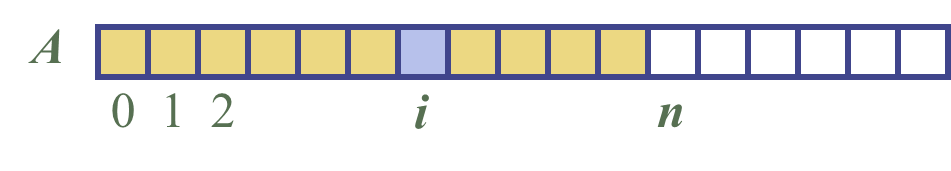
\includegraphics[width=9cm]{asp-04-pic01.png}
  \end{center}
\end{frame}


\begin{frame}[fragile]
  \frametitle{Nizovi karaktera / nizovi referenci na objekte}
  \begin{itemize}
    \item niz može da čuva primitivne elemente, na primer karaktere,
    predstavljajući \myred{kompaktni niz}
  \end{itemize}
  \begin{center}
    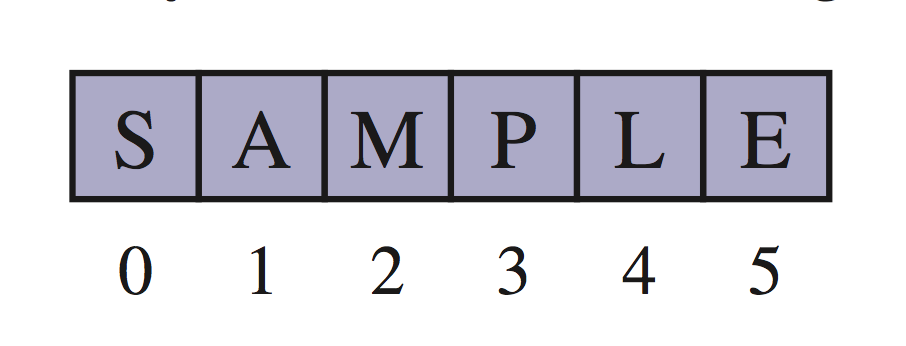
\includegraphics[width=4cm]{asp-04-pic02.png}
  \end{center}
  \begin{itemize}
    \item niz može čuvati i reference na objekte
  \end{itemize}
  \begin{center}
    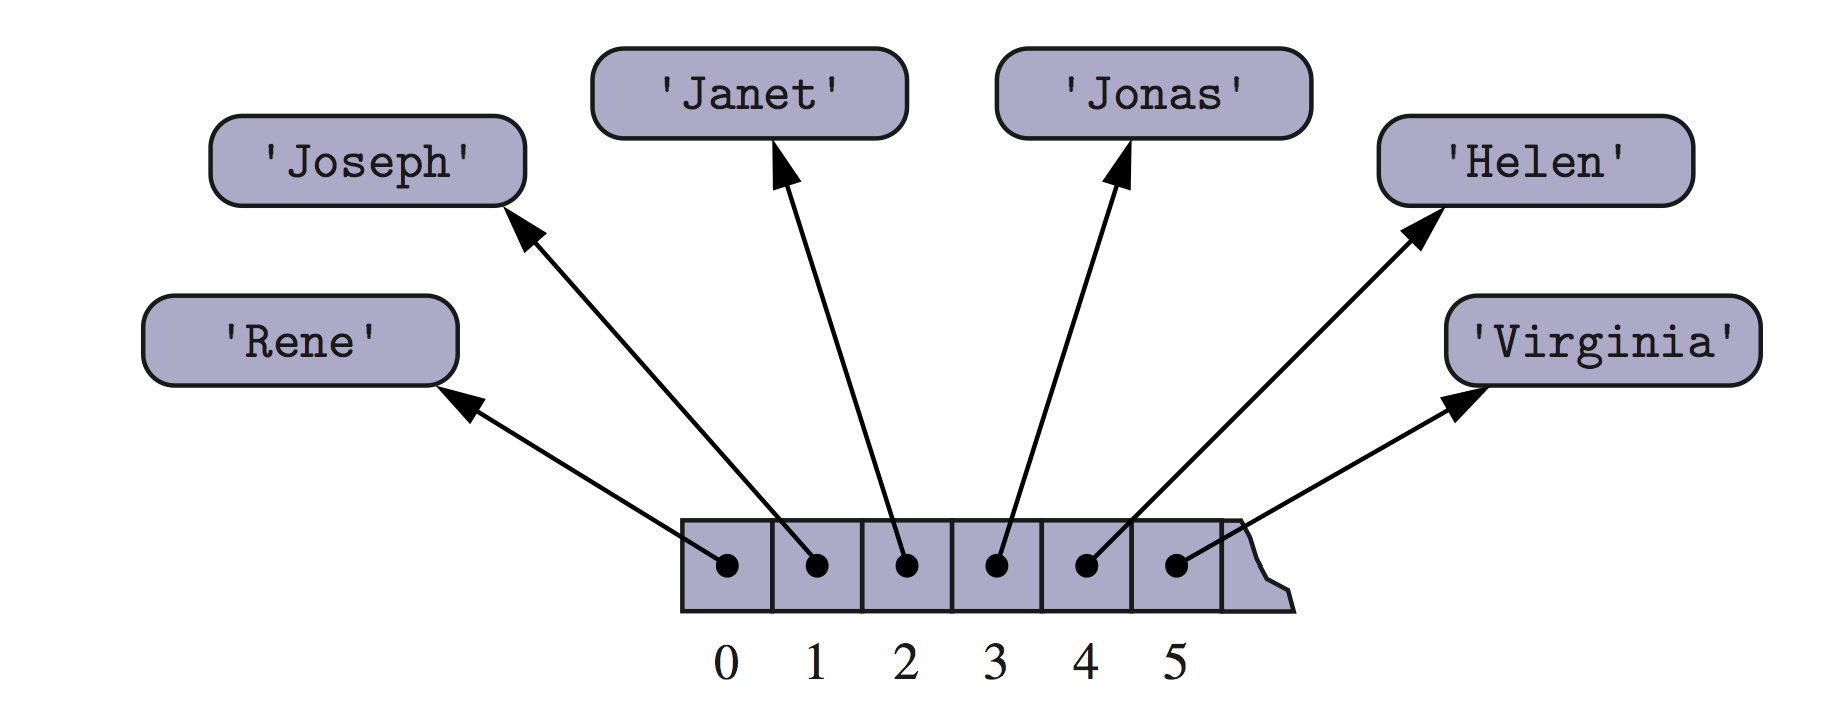
\includegraphics[width=8cm]{asp-04-pic03.png}
  \end{center}
\end{frame}

\begin{frame}[fragile]
  \frametitle{Kompaktni nizovi}
  \begin{itemize}
    \item podrška za rad sa kompaktnim nizovima nalazi se u modulu
    \texttt{array}
    \item ovaj modul definiše klasu \texttt{array} koja predstavlja kompaktni
    niz za primitivne tipove podataka
    \item konstruktor za \texttt{array} kao prvi parametar očekuje slovo koje
    označava tip elemenata
  \end{itemize}
\begin{minted}[linenos=false]{python}
primes = array('i', [2, 3, 5, 7, 11, 13, 17, 19])
\end{minted}
\end{frame}

\begin{frame}[fragile]
  \frametitle{Tipovi elemenata za \texttt{array}}
  \begin{itemize}
    \item klasa \texttt{array} prepoznaje sledeće oznake tipa elemenata
  \end{itemize}
\begin{center}
\begin{tabular}{clr}
\textbf{kod} & \textbf{tip podatka} & \textbf{veličina} \\
\hline \hline 
\texttt{'c'} & char & 1 \\ \hline 
\texttt{'b'} & signed char & 1 \\ \hline 
\texttt{'B'} & unsigned char & 1 \\ \hline
\texttt{'u'} & Unicode char & 2 \\ \hline
\texttt{'h'} & signed short int & 2 \\ \hline
\texttt{'H'} & unsigned short int & 2 \\ \hline
\texttt{'i'} & signed int & 2 \\ \hline
\texttt{'I'} & unsigned int & 2 \\ \hline
\texttt{'l'} & signed long & 4 \\ \hline
\texttt{'L'} & unsigned long & 4 \\ \hline
\texttt{'f'} & float & 4 \\ \hline
\texttt{'d'} & double & 8 \\ \hline
\end{tabular}
\end{center}
\end{frame}

\section[Operacije]{Operacije nad nizom}
\begin{frame}[fragile]
  \frametitle{Ubacivanje elementa}
  \begin{itemize}
    \item u operaciji \myred{add}($i, o$) treba napraviti mesta za novi element
    pomeranjem $n-i$ elemenata $A[i], \ldots, A[n-1]$ u desno za jedno mesto
    \item u najgorem slučaju ($i = 0$) za ovo je potrebno $O(n)$ vreme
  \end{itemize}
  \begin{center}
    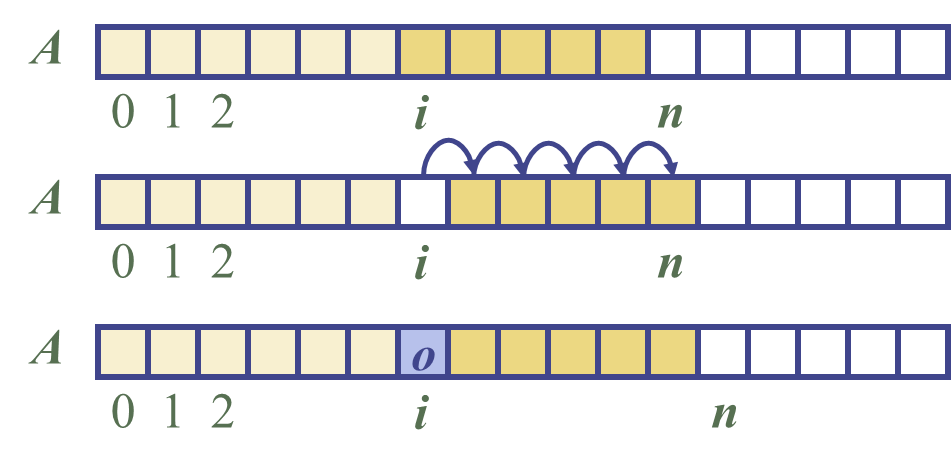
\includegraphics[width=9cm]{asp-04-pic04.png}
  \end{center}
\end{frame}

\begin{frame}[fragile]
  \frametitle{Uklanjanje elementa}
  \begin{itemize}
    \item u operaciji \myred{remove}($i$) treba popuniti rupu na mestu elementa
    koji se uklanja pomeranjem $n-i-1$ elemenata $A[i+1], \ldots, A[n-1]$ u
    levo za jedno mesto
    \item u najgorem slučaju ($i = 0$) za ovo je potrebno $O(n)$ vreme
  \end{itemize}
  \begin{center}
    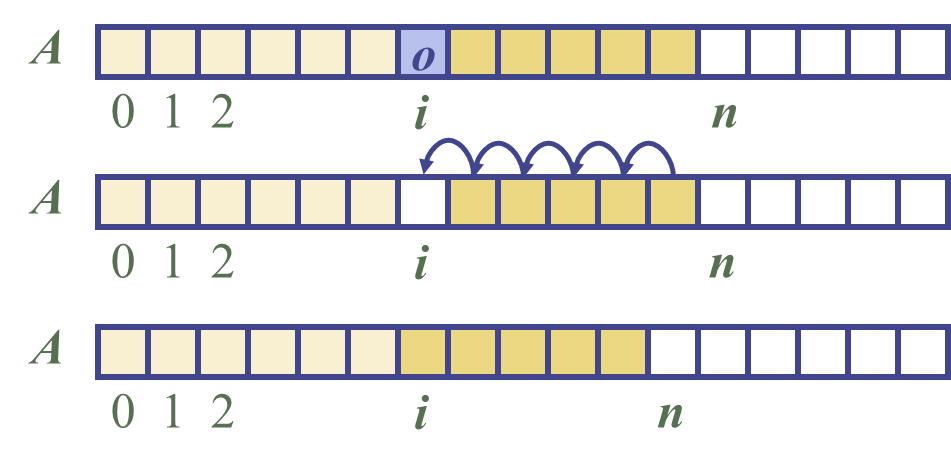
\includegraphics[width=9cm]{asp-04-pic05.png}
  \end{center}
\end{frame}

\begin{frame}[fragile]
  \frametitle{Performanse niza}
  \begin{itemize}
    \item za implementaciju liste pomoću niza
    \begin{itemize}
      \item prostor koji zauzima struktura u memoriji je $O(n)$
      \item pristup $i$-tom elementu je u $O(1)$ vremenu
      \item ubacivanje i uklanjanje su u $O(n)$ vremenu u najgorem slučaju
    \end{itemize}
  \end{itemize}
\end{frame}

\begin{frame}[fragile]
  \frametitle{Performanse niza}
  \begin{itemize}
    \item šta je zaista najgori slučaj kod dodavanja?
    \begin{itemize}
      \item niz popunjen do kraja
      \item zauzmemo novi (veći) niz u memoriji
      \item prepišemo sve podatke iz starog niza
      \item odbacimo stari niz
    \end{itemize}
    \item moramo unapred znati veličinu niza!
  \end{itemize}
\end{frame}

\section[Proširenje]{Proširenje niza}
\begin{frame}[fragile]
  \frametitle{Strategije za proširenje niza}
  \begin{itemize}
    \item koliko velik treba da bude novi niz prilikom proširenja?
    \begin{itemize}
      \item \myred{inkrementalna} strategija: novi niz će biti duži za neko
      konstantno $c$
      \item strategija \myred{dupliranja}: novi niz će biti duplo duži od
      prethodnog
    \end{itemize}
  \end{itemize}
\end{frame}

\begin{frame}[fragile]
  \frametitle{Poređenje strategija}
  \begin{itemize}
    \item poredimo strategije analizirajući ukupno vreme $T(n)$ potrebno za
    obavljanje $n$ operacija ubacivanja
    \item krećemo od niza dužine 1
    \item amortizovano vreme add operacije: prosečno vreme potreno za operaciju
    za niz od $n$ operacija, $T(n)/n$
  \end{itemize}
\end{frame}

\begin{frame}[fragile]
  \frametitle{Poređenje strategija: inkrementalna}
  \begin{itemize}
    \item pravimo novi niz $k = n/c$ puta
    \item ukupno vreme $T(n)$ za seriju od $n$ operacija ubacivanja je
    proporcionalno sa:
    $$ n + c + 2c + 3c + 4c + \ldots + kc = $$
    $$ n + c(1 + 2 + 3 + \ldots + k) = $$
    $$ n + ck(k+1)/2$$
    \item $c$ je konstanta, sledi da $T(n)$ je $O(n+k^2)$ odnosno $O(n^2)$
    \item $\Rightarrow$ amortizovano vreme operacije ubacivanja je $O(n)$
  \end{itemize}
\end{frame}

\begin{frame}[fragile]
  \frametitle{Poređenje strategija: dupliranje}
  \begin{itemize}
    \item pravimo novi niz $k = \log_2 n$ puta
    \item ukupno vreme $T(n)$ za seriju od $n$ operacija ubacivanja je
    proporcionalno sa:
    $$ n + 1 + 2 + 4 + 8 + \ldots + 2^k = $$
    $$ n + 2^{k+1} = $$
    $$ 3n - 1$$
    \item $T(n)$ je $O(n)$
    \item $\Rightarrow$ amortizovano vreme operacije ubacivanja je $O(1)$
  \end{itemize}
\end{frame}

\begin{frame}[fragile,shrink=15]
  \frametitle{Implementacija u Pythonu $_1$}
\begin{minted}[linenos=false]{python}
class DynamicArray:
  def __init__(self):
    self._n = 0                # stvarni broj elemenata
    self._capacity = 1         # kapacitet niza
    self._A = self._make_array(self._capacity) # zauzimanje niza
                                               # u memoriji
  def __len__(self):
    return self._n             # vrati broj elemenata
    
  def __getitem__(self, k):
    if not 0 <= k < self._n:
      raise IndexError('invalid index')
    return self._A[k]          # dobavi element po indeksu
\end{minted}
\end{frame}

\begin{frame}[fragile,shrink=15]
  \frametitle{Implementacija u Pythonu $_2$}
\begin{minted}[linenos=false]{python}
  def append(self, obj):
    if self._n == self._capacity:       # da li je niz popunjen?
      self._resize(2 * self._capacity)  # udvostruči mu kapacitet
    self._A[self._n] = obj
    self._n += 1
    
  def _resize(self, c):
    B = self._make_array(c)             # novi (veći) niz
    for k in range(self._n):            # prepiši vrednosti u njega
      B[k] = self._A[k]
    self._A = B
    self._capacity = c
    
  def _make_array(self, c):
    import ctypes
    return (c * ctypes.py_object)()     # pogledaj dok za ctypes
\end{minted}
\end{frame}

\end{document}
